\documentclass[pdflatex,sn-basic]{sn-jnl}
\usepackage{graphicx}
\usepackage{amsmath,amssymb}
\usepackage{booktabs,array}
\usepackage{placeins}
\hypersetup{pdftitle={Batch-dependent negative sampling and marginal-preserving decoy construction in TCR-peptide benchmarks},pdfauthor={Sharon Melhi and Rajat Bhardwaj}}
\newcommand{\TV}{\operatorname{TV}}
\newcommand{\AUC}{\operatorname{AUROC}}
\raggedbottom
\begin{document}
\title[Auditing TCR benchmark construction]{Batch-dependent negative sampling and marginal-preserving decoy construction in TCR--peptide benchmarks}
\author[1]{\fnm{Sharon} \sur{Melhi}}
\author*[1]{\fnm{Rajat} \sur{Bhardwaj}}\email{rajat@blr.amity.edu}
\affil[1]{\orgdiv{Amity School of Engineering and Technology}, \orgname{Amity University Bengaluru}, \orgaddress{\city{Bengaluru}, \country{India}}}
\abstract{Negative examples in T-cell receptor (TCR)--peptide benchmarks are often generated by recombining observed positive records. Such construction can introduce label contradictions and antigen-frequency shortcuts independently of a binding model. We audited an executable batch-based sampler on a frozen VDJdb release and evaluated a closed assignment within human leukocyte antigen (HLA) strata that excludes catalogued positive triples while preserving the retained empirical marginals. The primary human class-I cohort contained 3,182 distinct triples of receptor beta-chain complementarity-determining region 3, peptide and HLA. Across 30 sampling seeds, the source sampler generated catalogued-positive contradictions in 2.989\%, 0.882\% and 0.228\% of decoys under release-order, peptide-sorted and shuffled loading, respectively. On identical retained records, independent within-HLA rejection removed those contradictions but left mean peptide total variation of 0.135; closed assignment reduced both diagnostics to zero. This guarantee retained 2,691 records (84.57\%) and only 22 of 41 HLA strata. With receptor folds fixed before decoy construction, a peptide/HLA-only classifier achieved mean held-out-receptor area under the receiver operating characteristic curve of 0.556 for sorted loading and 0.500 for shuffled loading and assignment. Constructing globally before cross-validation instead produced complementary-fold artefacts. Higher confidence filtering and peptide-distance partitioning exposed additional feasibility limits. These results establish a reproducible construction audit and a constrained correction with an explicit coverage cost; they neither certify biological nonbinding nor demonstrate improved binding prediction.}
\keywords{T-cell receptor, negative sampling, benchmark integrity, HLA, constrained assignment, reproducibility}
\maketitle

\section{Introduction}\label{sec:intro}
Predicting which T-cell receptors recognize a peptide presented by a major histocompatibility complex is a central computational immunology problem. Models using paired receptor chains, contextual sequence embeddings and attention have expanded the available approaches \citep{Montemurro2021,Weber2021,Korpela2023}. Their evaluation, however, depends on the definition of a negative example. A database of experimentally supported recognition events does not ordinarily contain a complete, assay-matched set of nonbinding pairs. Recombining receptors and antigens supplies convenient decoys, but the resulting binary task includes properties introduced by the construction algorithm.

This concern is established rather than new. Dens et al. demonstrated the consequences of replacing background-repertoire negatives with shuffled observed sequences \citep{Dens2023}. Shuffling with known-partner exclusion and construction within predefined partitions already appear in prior work \citep{Moris2021,Korpela2023}. TEINet explicitly contrasted uniform epitope-category sampling with positive-frequency-weighted sampling and demonstrated frequency-induced apparent discrimination \citep{Jiang2023}. Broader assessments show that data sources and evaluation protocols strongly affect reported performance \citep{Deng2023,Drost2025,Lu2026}. Mi et al. investigated a different constructive strategy based on receptor junction mutations \citep{Mi2026}. Separately, receptor--peptide models often generalize poorly to unseen peptides, motivating explicit antigen holdout and distance-aware evaluation \citep{Grazioli2022,Castorina2025}. These studies establish the need to interrogate benchmark construction; they do not imply that every recombination algorithm obeys the same invariants.

We investigate a specific implementation-level failure pathway. A batch sampler initially permutes observed ligand rows, attempts to avoid assigning the same peptide, and falls back to a global pool of unique peptide--HLA values when local repair fails. Sampling records and sampling unique ligand categories are different distributions. Batch order can therefore change the generated label distribution even when every candidate sequence originates from the same database. A second, independent question is whether recorded positive triples are actually excluded. Avoiding the original peptide is insufficient when a receptor has several catalogued targets.

The study makes three bounded contributions. First, executable source tests and a fixed public-data audit separate registry contradictions from marginal distribution changes. Second, a standard assignment formulation yields a maximum-size \emph{closed subset of rows}, within each HLA stratum, for which registry exclusion and exact retained marginals can hold simultaneously. The algorithm's exclusion cost is measured rather than hidden. Third, trained metadata controls examine whether construction labels are learnable across held-out receptor groups, and a protocol-placement sensitivity demonstrates why negative construction should follow partitioning. The object of evaluation is the construction procedure, not a new biological binding predictor.

\section{Materials and methods}\label{sec:methods}
\subsection{Public data, eligibility and target definition}
We used the VDJdb release dated 1 June 2023 \citep{Shugay2018}, preserving its original archive and recording SHA-256 checksums. The release contains 92,771 rows. We sequentially retained human records, TRB chains, class-I MHC entries, source labels matching two-field HLA-A/B/C syntax, canonical CDR3-beta sequences beginning with C and ending with F or W, and canonical peptides of length 8--15. This HLA filter checks syntax, not nomenclature validity; ``HLA strata'' below denote source-annotation strata. No missing HLA value was imputed or converted to a presumed allele. The resulting 35,237 rows were filtered by database confidence score and deduplicated by the exact tuple $(b,p,h)$, where $b$ denotes CDR3-beta, $p$ peptide and $h$ the source HLA label (Table~\ref{tab:cohort}). Deduplication retained the first eligible source row, with zero-based source identifiers saved for reconstruction. An additional annotation sensitivity excluded two flagged HLA labels from both cohorts and the reference registry, without recoding.

The primary positive cohort required score $\geq1$. Sensitivity cohorts used all scores and score 3 only. The exclusion reference $K$ contained every eligible tuple across all scores, including score 0. This broader reference was used to flag avoidable contradictions, not to certify the strength of every underlying assay. We also recomputed contradiction rates using a score-$\geq1$ reference. Throughout, a \emph{registry contradiction} means that a generated negative tuple occurs in the declared reference. Because the target key omits the alpha chain, V/J genes and full receptor context, this quantity is not an experimentally measured false-negative rate for complete alpha--beta receptors. Generated pairs absent from $K$ remain unobserved pairs of unknown binding status.

\begin{table}[t]
\caption{Eligible cohorts after tuple deduplication. The 35,237 eligible source rows are shared before confidence filtering. Scores are the database's evidence annotations, not calibrated binding probabilities.}\label{tab:cohort}
\centering
\begin{tabular}{lrrrr}
\toprule
Confidence rule & Positive tuples & CDR3-beta & Peptides & HLA strata\\
\midrule
Score $\geq0$ & 29,306 & 27,078 & 927 & 41\\
Score $\geq1$ (primary) & 3,182 & 3,061 & 253 & 41\\
Score $=3$ & 320 & 308 & 38 & 11\\
\bottomrule
\end{tabular}
\end{table}

\subsection{Executable sampler audit and experimental controls}
The audited sampler is one research-code implementation, not a representative survey of the field. It receives a positive registry and a pool of distinct peptide--HLA values. Its class body was extracted through Python's abstract syntax tree and executed without changing the selection logic. Identity-tag embeddings and a NumPy tensor shim replaced numerical feature loading and tensor assembly. This executes sequence selection, including fallback branches, but does not execute a neural model or test numerical equivalence of neural features. Source fingerprints and the exact implementation are included in the public reproducibility archive; the mathematical behavior is specified here and in Online Resource 1.

For batches of size greater than one, the sampler constructs an index derangement and attempts swaps to remove equal-peptide assignments. If repair fails for a row, it samples a different peptide from the unique-ligand pool, with at most 20 attempts before a hard-coded sentinel. Singleton batches also use fallback. Whole peptide--HLA values are reassigned, so the receiver's original HLA need not be preserved. The supplied positive registry is stored but never read by this class. We verified that supplying an empty registry leaves a constructed cross-reactivity example unchanged, and that a single-peptide pool reaches the sentinel branch. These are executable source counterexamples, not estimates of their frequency in biological cohorts.

For each public cohort, we compared release order, lexical peptide order and a random row permutation. The primary batch size was 64; sizes 16 and 256 were additional primary-cohort sensitivities. Each stochastic configuration used 30 seeds. Row-order randomness and source-sampler randomness were separate; the global fallback pool retained fixed release order in every comparison. Each positive supplied one negative receptor copy, yielding balanced constructed classes. The source sampler was also rerun on the exact 2,691-row subset retained by the assignment procedure, providing a common-population comparison.

An independent rejection reference used that same retained population. For each receptor row it sampled, with replacement, uniformly among donor \emph{rows} in the same HLA stratum whose tuple was absent from $K$. This is equivalent to drawing uniform donor rows until an admissible row is accepted. Feasibility is guaranteed on this subset by the assignment solution. It distinguishes independent from coordinated donor selection under shared HLA and exclusion constraints; it is not an official published binding model. Comparisons of the source sampler with assignment change several constraints together and do not isolate marginal coordination alone. Thirty seeds were used, and the exact expected peptide distribution was computed from the admissible-row probabilities.

A separate synthetic experiment isolated the fallback mechanism. It contained 4,096 records, nine peptides, one peptide occupying half the records and eight peptides occupying one sixteenth each. At batch size 64, a prespecified score equal to one for the majority peptide and zero otherwise was evaluated across 100 sampler seeds. This score uses no training labels or receptor information. An exact cyclic reassignment preserving peptide counts provided a construction control.

\subsection{Construction diagnostics}
For $n$ positives and $n$ generated decoys, the registry-contradiction rate is the fraction of negative tuples in $K$. For a categorical feature $g$, let $N_+(c)$ and $N_-(c)$ be its positive and negative counts. We measured
\begin{equation}
\TV_g=\frac{1}{2n}\sum_c\left|N_+(c)-N_-(c)\right|.
\label{eq:tv}
\end{equation}
Features comprised receptor identity, peptide identity, HLA and joint peptide--HLA identity. A category-frequency \emph{identity oracle} assigned score $N_+(c)/(N_+(c)+N_-(c))$ on the same constructed dataset. Its area under the receiver operating characteristic curve (AUROC), with ties contributing one half, measures available marginal label separation. It is deliberately a resubstitution diagnostic, not a held-out prediction result. The trained controls below provide a separate evaluation.

If the positive and negative multisets of $g$ are identical, every fixed deterministic score $f(g)$ has identical class-conditional score distributions and AUROC $0.5$. This statement follows directly by exchanging a positive--negative pair, including ties. It does not imply that a cross-fitted model with different fitted scores in different folds must have pooled AUROC $0.5$ when equality is imposed only globally. Receptor-only chance performance is also structurally expected when every receptor is copied once into each class; it cannot establish learned molecular interaction.

\subsection{Closed within-HLA assignment with explicit abstention}
Consider one HLA stratum with positive rows $i=1,\ldots,n$. A donor row $j$ supplies its peptide to receptor $b_i$. Define an admissible off-diagonal edge by $(b_i,p_j,h)\notin K$. Because each original tuple occurs in $K$, this also excludes reassigning the same peptide to its original receptor. We solve a full linear assignment with cost
\begin{equation}
C_{ij}=\begin{cases}
1, & i=j\quad\text{(abstention)},\\
0, & i\ne j\ \text{and }(b_i,p_j,h)\notin K,\\
n+1, & \text{otherwise}.
\end{cases}
\label{eq:assignment}
\end{equation}
The SciPy solver, implementing a modified Jonker--Volgenant assignment algorithm \citep{Crouse2016}, minimizes $\sum_i C_{i,\pi(i)}$ over permutations $\pi$. Fixed points are discarded; each nonfixed row supplies its original positive tuple and the generated decoy $(b_i,p_{\pi(i)},h)$.

The identity permutation costs $n$, whereas any forbidden edge alone costs $n+1$. Consequently an optimal solution contains no forbidden edge. Its total cost equals its number of fixed points, so minimizing cost maximizes the number of retained rows under this contract. The nonfixed indices form permutation cycles: retained receptor-side and donor-side row sets are identical. This preserves receptor, peptide, HLA, receptor--HLA and peptide--HLA empirical marginals within the retained population. It does not preserve the original population when rows are excluded, does not guarantee unique negative tuples, and does not optimize all possible weighted or replacement-based resampling designs.

Assignment and matching are standard combinatorial tools \citep{Hall1935}; the contribution here is the explicit benchmark contract and its measured consequences. Ordinary maximum bipartite matching is only an upper bound on retained \emph{closed} rows. A directed path of three rows permits two matched edges but no nontrivial closed cycle. Independent exhaustive enumeration tested optimality and all certificates on 166 fixtures with one to eight rows, including repeated receptor and peptide identities and multiple HLA strata. Dense cost matrices have quadratic storage in stratum size; we make no large-repertoire scalability claim.

\subsection{Partition-aware trained metadata controls}
We assigned exact CDR3-beta groups to five folds before constructing decoys, using five fold seeds (17, 41, 73, 107 and 211). The assignment procedure was applied independently inside each fold. All source-sampler comparisons then used the same retained positives in that fold, at batch size 64, with ten decoy seeds. The registry $K$ remained a frozen retrospective sanitation reference; it was never supplied as a predictive feature. Antigen identities could recur across folds, while receptor identities could not.

Separate logistic regressions used peptide identity, HLA identity, their concatenated one-hot features, or receptor identity alone. Encoders were fitted only on the four training folds; unseen test categories were ignored. Hyperparameters were fixed: L2 regularization, $C=1$, \texttt{liblinear}, tolerance $10^{-8}$ and at most 2,000 iterations. Convergence warnings were treated as failures. No test-label tuning, threshold selection or score inversion was performed. We report pooled out-of-fold AUROC for each complete five-fold run, along with average precision and Brier scores in the supplement. These controls ask whether constructed labels are learnable within an antigen collection across unseen receptors. They are not unseen-peptide or clinical binding evaluations.

An initial, separately retained sensitivity constructed negatives globally on the 2,691-row common cohort and only then assigned receptor folds. This order can couple the class counts of complementary folds. The corrected primary protocol above was added after that diagnostic revealed below-chance results. Both are reported, and the study is exploratory rather than preregistered. Changing construction placement also changes feasible retention and batch composition; the difference between protocols is not interpreted as a single-factor causal effect.

\subsection{Distance-separated construction and statistical scope}
For a distinct construction sensitivity, we calculated unit-cost Levenshtein distances between all 253 primary-cohort peptides. Edges joined pairs at distance $\leq2$, and entire connected components were assigned to train, validation and test partitions. Each of five split seeds assigned 132, 44 and 45 of the 221 components, respectively; row fractions were allowed to vary. We verified every cross-partition peptide distance. Negative construction was then performed using candidate antigens from the relevant test partition, both on its full positives and its common retained subset. This examines feasibility after distance separation, without fitting a binding model. The global registry rejects known tuples but does not import external candidate peptides into a partition.

Means and standard deviations over decoy seeds describe conditional construction randomness on frozen data. They are not biological confidence intervals. For trained controls, each decoy-seed value first averages the five fold-seed runs; reported standard deviations summarize those ten averages. Ranges over all 50 runs additionally describe partition variation. The deterministic assignment has no sampling-seed standard deviation. We report effect sizes and complete run records without pair-level significance tests that would assume independent observations. Analyses used Python 3.12, NumPy, pandas, SciPy and scikit-learn; pinned versions, source-row manifests, raw aggregate outputs and figure scripts accompany the manuscript. ChatGPT assisted source inspection, code development, execution of computational analyses, literature searches, reviewer-role stress testing and manuscript drafting. Figures were drawn programmatically from the archived measurements. Executed code and archived outputs provide the numerical evidence; AI-generated reviewer reports are internal checks, not journal peer review. The human authors remain responsible for verifying the evidence and interpretation and approving submission.

\section{Results and discussion}\label{sec:results}
\subsection{Batch fallback creates a measurable peptide shortcut}
The synthetic experiment established a failure pathway without a fitted binding predictor (Fig.~\ref{fig:mechanism}). With sorted batches, all rows reached the unique-ligand fallback. The majority peptide accounted for approximately 6.25\% of negatives despite representing 50\% of positives, yielding fixed-score AUROC $0.7187\pm0.0016$. Shuffling reduced fallback to 4.92\% and AUROC to $0.5246\pm0.0023$. The exact cyclic control returned $0.5000$. These results demonstrate sensitivity to the sampler's accepted distribution; they do not estimate a neural network's biological accuracy.

\begin{figure}[t]
\centering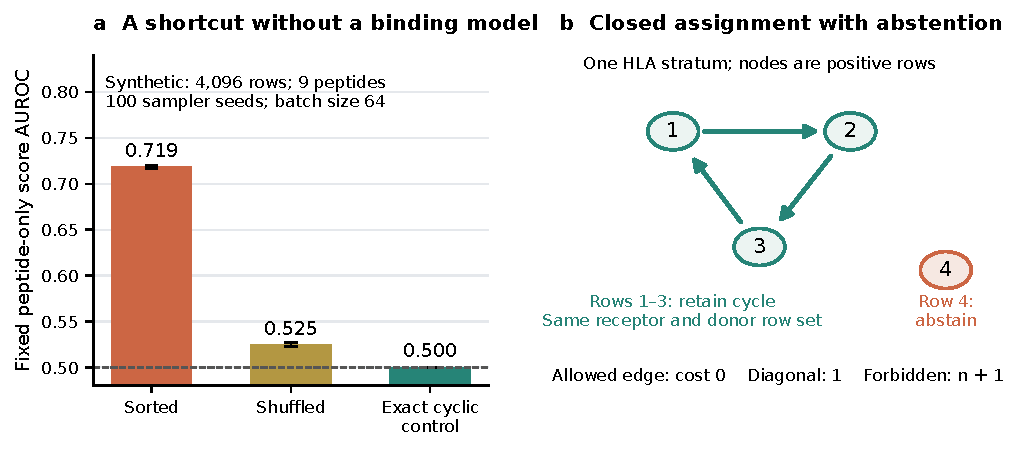
\includegraphics[width=\textwidth]{figures/Fig1.pdf}
\caption{Mechanism and constrained construction. (a) A fixed majority-peptide score in the declared synthetic experiment; error bars are standard deviations across 100 sampler seeds. The cyclic control preserves peptide counts exactly. (b) A schematic within-HLA closed assignment. Nodes represent positive rows; the illustrated admissible cycle retains rows 1--3, while row 4 is an abstention. This is a conceptual four-row example, not a biological interaction network.}\label{fig:mechanism}
\end{figure}

On the complete primary public cohort, release-order, peptide-sorted and shuffled loading generated registry contradictions in $2.9887\pm0.1022\%$, $0.8820\pm0.0761\%$ and $0.2284\pm0.0695\%$ of decoys, respectively. Here the standard deviations are percentage points. Corresponding peptide total variations were 0.1294, 0.4342 and 0, and identity-oracle AUROCs were 0.6048, 0.7916 and 0.5000. Thus marginal separation and registry contradictions are different diagnostics: sorting increased the former but reduced the latter relative to release order. A low contradiction rate alone does not establish a balanced construction.

Shuffling was an effective marginal control in this main cohort: peptide total variation was zero for every tested seed at batch sizes 16, 64 and 256 (Supplementary Fig.~S1). It nevertheless left registry contradictions. This is evidence for a useful simple control, not grounds to claim that only the assignment method can eliminate observed peptide-frequency bias.

\subsection{Exclusion alone and exact marginal control have different consequences}
The assignment retained 2,691 primary positives. Every common-cohort comparison used precisely these records (Table~\ref{tab:common}; Fig.~\ref{fig:common}). The source sampler still generated contradictions under all three loading regimes. Independent within-HLA rejection removed them entirely but produced peptide total variation $0.1349\pm0.0059$ and identity-oracle AUROC $0.5990\pm0.0038$. Its exact expected peptide total variation was 0.1020, showing that the imbalance is not solely finite-sample fluctuation. Receptor-specific admissibility changes the accepted donor distribution.

The closed assignment had zero registry contradictions and exact equality of every declared marginal. Its identity-oracle AUROC was therefore 0.5 by construction. All 166 exhaustive fixtures passed, comprising 924,960 enumerated permutations. The interpretation is a verified construction contract, not a victory on a predictive task. The assignment generated 2,624 unique negative tuples among 2,691 rows; repeated identities can yield duplicate output tuples despite a permutation of donor rows. Rejection generated a mean of 2,656.7 unique negative tuples. Exact marginal preservation therefore does not imply greater pair diversity.

\begin{table}[t]
\caption{Common-population audit on 2,691 retained positives, with one decoy per positive. Entries are means over 30 sampler seeds; selected standard deviations are shown after $\pm$, and full summaries accompany the analysis. The assignment is deterministic. The identity oracle uses the evaluated category counts and is not a prediction metric.}\label{tab:common}
\centering\small
\begin{tabular}{lrrr}
\toprule
Construction & Contradictions (\%) & Peptide TV & Oracle AUROC\\
\midrule
Source: release order & $2.532\pm0.109$ & $0.1211$ & $0.5942$\\
Source: peptide sorted & $0.684\pm0.069$ & $0.3779$ & $0.7611$\\
Source: row shuffled & $0.256\pm0.089$ & $0.000012$ & $0.500012$\\
Within-HLA rejection & $0$ & $0.1349\pm0.0059$ & $0.5990\pm0.0038$\\
Closed assignment & $0$ & $0$ & $0.5000$\\
\bottomrule
\end{tabular}
\end{table}

\begin{figure}[t]
\centering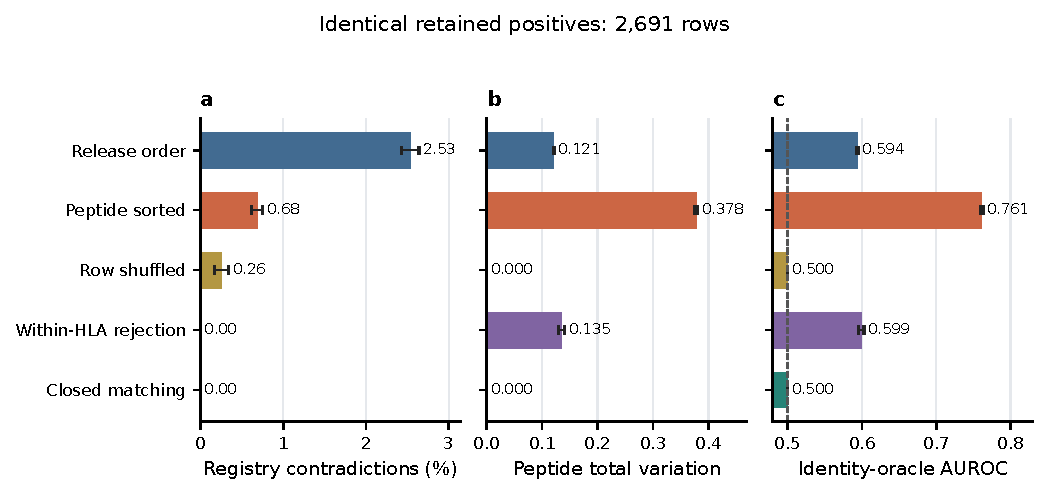
\includegraphics[width=\textwidth]{figures/Fig2.pdf}
\caption{Registry exclusion and marginal balance on identical retained positives. Panels compare contradiction rate, peptide total variation and peptide identity-oracle AUROC. Error bars show sampler-seed standard deviations; some are smaller than the drawn marks. Independent rejection excludes registered positives but does not enforce the peptide marginal. The matching result is a construction identity, not evidence of superior biological prediction.}\label{fig:common}
\end{figure}

\subsection{Confidence filtering changes the feasibility problem}
Evidence thresholds changed both contradiction rates and marginal behavior (Fig.~\ref{fig:confidence}). The all-score cohort had a shuffled contradiction rate of 5.1545\%, whereas the score-3 cohort had a rate of 0.09375\%. However, the latter cohort concentrated 186 of 320 rows (58.125\%) on one peptide. Even globally, a no-identical-peptide permutation retaining all rows is impossible when one peptide occupies more than half the rows: its receivers outnumber the available different-peptide donors. Within-HLA and cross-reactivity restrictions can further reduce feasibility.

Consequently shuffled loading in the score-3 cohort still produced mean peptide total variation 0.1671 and identity-oracle AUROC 0.6069. Its within-HLA assignment retained only 139 rows (43.44\%). More restrictive evidence filtering does not automatically yield a less biased decoy task; it can increase antigen concentration. Registry confidence also matters independently. Restricting $K$ to score-$\geq1$ entries lowered the primary source-sampler contradiction rates to 2.6639\%, 0.8003\% and 0.1446\%, but did not remove the problem. Assignment against that narrower registry retained 2,696 rows and produced eight contradictions against the broader registry. These are reference-dependent audit outcomes, not estimates of hidden biological binding.

\begin{figure}[t]
\centering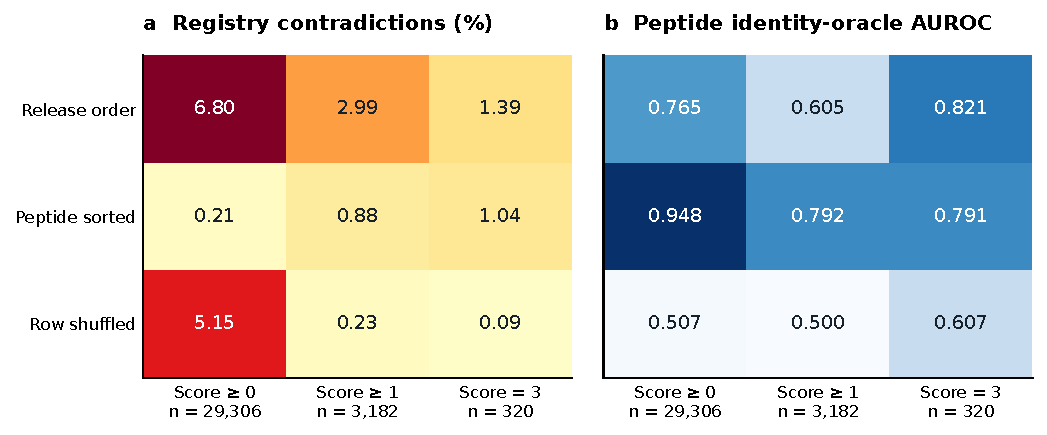
\includegraphics[width=\textwidth]{figures/Fig3.pdf}
\caption{Confidence sensitivity on full positive cohorts, before assignment-based exclusions. Values average 30 source-sampler seeds at batch size 64. (a) Registry-contradiction percentages against all eligible evidence scores. (b) Peptide identity-oracle AUROC. The shuffled score-3 result illustrates why a useful randomization control in one cohort need not guarantee marginal balance in another.}\label{fig:confidence}
\end{figure}

\subsection{Coverage is the cost of the exact construction contract}
The primary assignment retained 84.57\% of rows, 236 of 253 peptides and 22 of 41 source HLA strata. Nineteen source strata were lost entirely. The HLA-distribution total variation between original and retained positives was 0.1274. This selection is part of the result, not missing data to be ignored (Fig.~\ref{fig:coverage}). In the HLA-B*27:05 stratum, 38 of 130 rows formed a closed admissible subset; ordinary maximum bipartite matching allowed 49 edges. The 11-row difference illustrates the extra restriction required to keep the positive receiver and ligand donor populations identical.

Annotation review against the frozen IPD-IMGT/HLA 3.52.0 nomenclature identified two source labels without an active matching two-field prefix: HLA-A*08:01 (two records) and the deleted legacy HLA-A*24:01 (72 records). Removing both without reassignment left 3,108 positives and 39 source strata; assignment retained 2,665 rows (85.75\%) and 21 strata, with unchanged certificates. The retained manifest exactly equalled the original assignment with the affected stratum removed. In a rerun of 30 seeds per loading regime, source contradiction rates remained 2.888\%, 0.933\% and 0.245\%, and peptide-oracle AUROCs were 0.6423, 0.7936 and 0.5000 for release, sorted and shuffled order. Removing records also changes batch composition, so these shifts are not attributed to an allele's biology. Independently regenerated receptor folds and metadata models gave sorted AUROC 0.5619, release-order AUROC 0.5188, and 0.5000 for shuffling and assignment. Supplementary Methods document the nomenclature evidence and reruns.

Distance separation further reduced feasible coverage. All five component partitions had minimum cross-partition Levenshtein distance 3, confirming their stated separation. Their test sets contained 372--1,022 positives, and assignment retained 32.04--72.85\% (Supplementary Table~S2). Every corrected subset retained its construction certificates, but it represented a substantially smaller antigen/HLA population. A benchmark can therefore have valid sequence separation while still facing a difficult negative-construction problem. Neither split integrity nor exact marginals substitutes for reporting which biological strata remain evaluable.

\begin{figure}[t]
\centering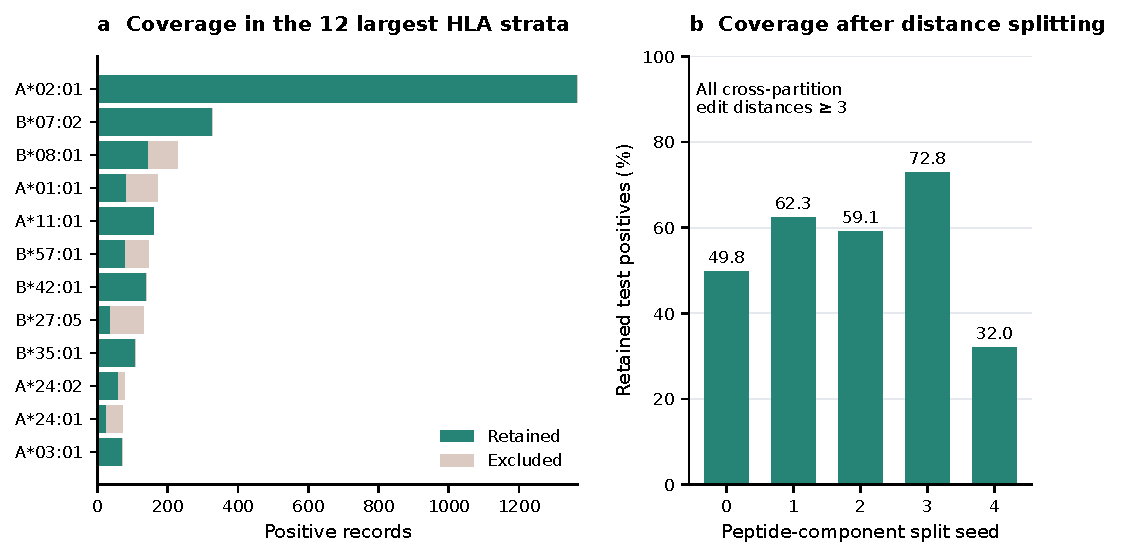
\includegraphics[width=\textwidth]{figures/Fig4.pdf}
\caption{Coverage costs of the closed assignment. (a) Retained and excluded positives in the 12 largest HLA strata of the primary cohort; complete values for all 41 strata accompany the analysis. (b) Retention within the test partition of each independently generated peptide-component split. These partitions satisfy pairwise cross-partition edit distance at least 3; they are construction sensitivities, not trained unseen-peptide benchmarks.}\label{fig:coverage}
\end{figure}

\subsection{Trained metadata controls depend on construction placement}
With folds fixed first, the five fold assignments retained 2,667, 2,659, 2,652, 2,670 and 2,658 positives, respectively. All samplers used identical positives within each fold assignment. Peptide-plus-HLA logistic regression achieved AUROC $0.5558\pm0.0011$ under peptide-sorted loading, with a range of 0.5435--0.5633 over all 50 runs. Release-order loading achieved $0.5168\pm0.0006$; shuffled loading and the closed assignment both gave 0.5000 (Fig.~\ref{fig:placement}a). The receptor-only control returned 0.5 in every configuration. This establishes modest, reproducible learnability of construction labels without receptor input in the sorted condition. It does not establish biological recognition or superiority of assignment over shuffling on this marginal diagnostic.

The global-construction sensitivity produced a different pattern. Sorted loading yielded mean metadata AUROC 0.7146, but globally shuffled and matched datasets yielded 0.3298 and 0.3262, respectively (Fig.~\ref{fig:placement}b). These below-chance values were retained without flipping scores. If a category is globally class-balanced, its held-out count imbalance is exactly the negative of its training imbalance:
\begin{equation}
\Delta_{\mathrm{test}}(c)=-\Delta_{\mathrm{train}}(c),\qquad
\Delta(c)=N_+(c)-N_-(c).
\end{equation}
A fitted category model can therefore learn an ordering opposite to the held-out imbalance. Enforcing balance before splitting can create finite-dataset dependence even when receptor groups are disjoint. Enforcing the declared construction separately inside frozen partitions avoids this particular coupling. The two protocols also differ in retained rows and batch composition, so their overall AUROC difference should not be assigned entirely to this mechanism.

\begin{figure}[t]
\centering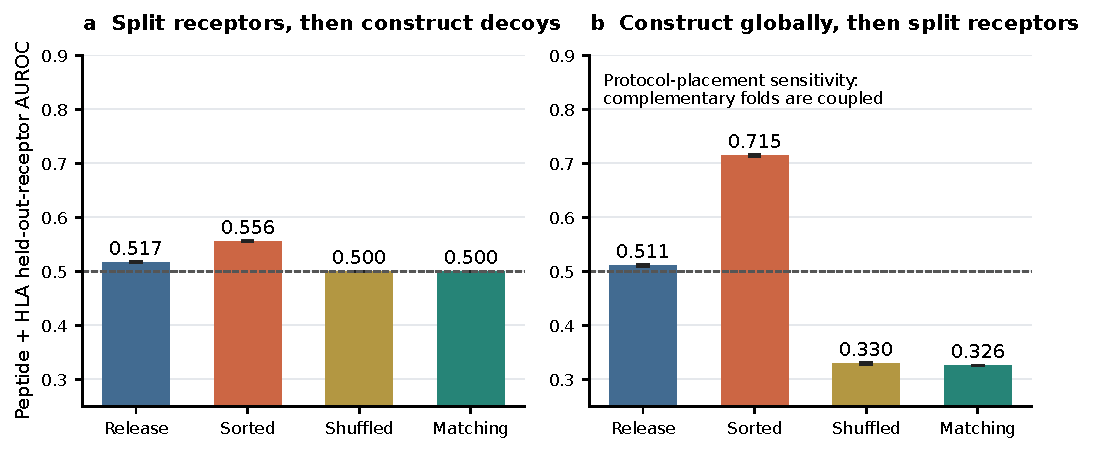
\includegraphics[width=\textwidth]{figures/Fig5.pdf}
\caption{Trained peptide-plus-HLA controls with no receptor features. (a) Primary protocol: split exact receptor groups, then construct decoys separately inside each fold. (b) Sensitivity: construct globally, then split receptor groups. Bars average five fold assignments and ten source-sampler seeds; matching is deterministic for a given cohort. Error bars summarize variation among decoy-seed means, not biological uncertainty. Protocols have different feasible retained populations; the comparison is descriptive. Below-chance values in (b) expose complementary-fold coupling and are not biological reverse prediction.}\label{fig:placement}
\end{figure}

\subsection{Implications and limitations}
The results refine an established negative-data-bias concern rather than introduce it. Prior work has already shown that apparently strong TCR prediction may reflect data origin, seen-antigen evaluation or negative construction \citep{Dens2023,Jiang2023,Lu2026,Castorina2025,Mi2026}. Here, a fallback from row permutation to sampling unique ligand categories provides a concrete, executed mechanism inside one sampler. Registry exclusion, retained marginal equality, population coverage and partition placement must be checked separately. The independent rejection comparator is useful precisely because it passes the first check while failing the second.

This audit covers one implementation and one frozen registry; applicability to other pipelines remains to be tested. Registry exclusion does not establish biological nonbinding, and beta-chain records omit full receptor context. Exact marginals apply to retained records, so the reported loss of rows and HLA coverage matters when interpreting the benchmark. Other shortcuts can remain. The metadata controls test construction signals; interaction-aware models and assay-confirmed nonbinders are needed to assess biological generalization. Alternative assignments, duplicate tuples and solver scaling are discussed in Online Resource 1.

Building on earlier partition-first generation \citep{Korpela2023}, the practical recommendation is to publish a construction manifest and explicit postconditions: fixed biological eligibility; partitions defined before candidate generation; declared positive-reference scope; measured registry contradictions; marginal and duplicate audits; and retention by peptide and HLA. A simple shuffled sampler may already pass some of these checks. When the closed-assignment contract is desired, infeasibility should be represented as an explicit exclusion rather than an undocumented fallback. The reported coverage cost is essential to deciding whether that contract is appropriate for a particular scientific question.

\section{Conclusions}
An executable batch-based sampler generated registry contradictions and order-dependent antigen-frequency signals on a versioned public TCR dataset. Independent positive exclusion removed contradictions while leaving marginal imbalance. A closed within-HLA assignment enforced both properties on a maximum retained row subset, with a substantial and measurable loss of rows and HLA coverage. Receptor-grouped metadata controls confirmed a modest sorted-batch shortcut and exposed the importance of partitioning before decoy construction. These findings support auditable benchmark construction with explicit feasibility limits; they do not validate a biological nonbinding label or a superior binding predictor.

\backmatter
\bmhead{Supplementary information}
Online Resource 1 (\texttt{ESM\_1.pdf}) provides supplementary methods and results, including filtering details, complete protocol settings, assignment certificates and sensitivity analyses. The public reproducibility archive contains source-row manifests, analysis programs, aggregate measurements, prediction records and vector figures, with original licenses and source provenance preserved.
\bmhead{Statements and declarations}
\textbf{Data and code availability.} VDJdb release 2023-06-01 is available at \url{https://github.com/antigenomics/vdjdb-db/releases/tag/2023-06-01}. Reconstruction uses the untouched source release and source-row manifests rather than redistributed modified sequence tables. All analysis code, generated measurements and the pinned audited source are available in the \texttt{benchmark\_audit} directory of \url{https://github.com/Sharon-codes/Precision-Oncology}, at frozen research revision \texttt{a4162ded50ba24d76ab8d5134577eba6935f910b}. The repository includes checksum-verified restoration of large prediction files and complete reproduction instructions.\par
\textbf{Ethics scope.} This computational study reanalyses public database records and generates synthetic decoys; no new participant recruitment, specimens or animal experiments were undertaken.\par
\textbf{Funding, competing interests and author contributions.} These author-specific declarations await confirmation and must be completed before journal submission. No absence of funding or competing interests, or allocation of human contributions, is inferred from the computational record.
\setlength{\bibsep}{0.45em}
\bibliography{references}
\end{document}
